% Den boolschen Wert false als Kommando \FALSE darstellen
\newboolean{boolfalse}
\setboolean{boolfalse}{false}
\newcommand{\FALSE}{\boolean{boolfalse}}

% Den boolschen Wert true als Kommando \TRUE darstellen
\newboolean{booltrue}
\setboolean{booltrue}{true}
\newcommand{\TRUE}{\boolean{booltrue}}

%\boolparam wird ben\"otigt, da #1 im END-Bereich nicht verf\"ugbar
\newcommand*{\boolparam}{}

\newcommand{\bild}[3]{
  \begingroup
    \par
    \setcapindent*{-0em}
    \setcapwidth[o]{0.15\linewidth}
    \settoheight{\bildhoehe}{\includegraphics[scale=#3]{#2}}
    \addtolength{\bildhoehe}{-3em}
    \addvspace{\baselineskip}
  \begin{figure}[h!t]
    \begin{captionbeside}{#1}[o][\linewidth][4.3em]*
      \parbox[t][\bildhoehe][b]{0.85\linewidth}{
      \centering\includegraphics[scale=#3]{#2}}
    \end{captionbeside}
    \label{#2}
  \end{figure}
    \par
  \endgroup
}

\newsavebox{\litbox}

\newenvironment{literaturbuch}{
  \marginpar{\vspace{1em}\ifthispageodd{\hspace*{-4em}}{\hspace*{3em}}
\includegraphics[scale=1]{buch}}
  \begin{lrbox}{\litbox}
    \begin{minipage}{.975\linewidth}
      \begin{small}
        \begin{itemize}
}{
        \end{itemize}
      \end{small}
    \end{minipage}
  \end{lrbox}
  \par\fbox{\usebox{\litbox}}\par
}

\newenvironment{merke}{
  \par
  \leaders\vbox to 2\baselineskip{%

  }\vskip2\baselineskip
  \marginpar{\vspace*{-1.5em}\ifthispageodd{\hspace*{1em}}{\hspace*{3em}}
\includegraphics[scale=1]{gluehbirne}}
  \vspace{-1.5em}
  \begin{lrbox}           {\litbox}
    \begin{minipage}{.96\linewidth}
}{
    \end{minipage}
  \end{lrbox}
  \fbox{\colorbox{lightyellow}{\usebox{\litbox}}}
  \par
  \addvspace{\baselineskip}
}

\newenvironment{literaturinternet}{
  \par
  \leaders\vbox to 2\baselineskip{%

  }\vskip2\baselineskip
  \marginpar{\vspace*{-1.5em}\ifthispageodd{\hspace*{1em}}{\hspace*{3em}}
\includegraphics[scale=1]{globus}}
  \vspace{-1.5em}
  \begin{lrbox}{\litbox}
    \begin{minipage}{.96\linewidth}
      \begin{small}
        \begin{itemize}
}{
        \end{itemize}
      \end{small}
    \end{minipage}
  \end{lrbox}
  \fbox{\usebox{\litbox}}
  \par
  \addvspace{\baselineskip}
}

%isTable=true, weil das Symbol meist vor Tabellen benutzt wird
\newboolean{isTable}
\setboolean{isTable}{true}
\newenvironment{oraclesql}[1][\boolean{isTable}]{
  \renewcommand*{\boolparam}{#1}
  \par
  \leaders\vbox to 2\baselineskip{%

  }\vskip2\baselineskip
  \marginpar{\vspace*{-1.5em}\ifthispageodd{\hspace*{1em}}{\hspace*{3em}}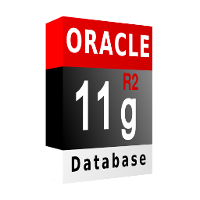
\includegraphics[scale=1]{oracle_11g}}
  \ifthenelse{\boolparam} {
    \vspace{-1.5em}
  } {
    \vspace{-3.5em}
  }
  \begin{lrbox}{\litbox}
    \begin{minipage}{.96\linewidth}
}{
    \end{minipage}
  \end{lrbox}
  \usebox{\litbox}
  \ifthenelse{\boolparam} {
  \par
  \addvspace{\baselineskip}
  } {
  }
}

\newenvironment{mssql}[1][\boolean{isTable}]{
  \renewcommand*{\boolparam}{#1}
  \par
  \leaders\vbox to 2\baselineskip{%

  }\vskip2\baselineskip
  \marginpar{\vspace*{-1.5em}\ifthispageodd{\hspace*{1em}}{\hspace*{3em}}
\includegraphics[scale=1]{ms_sql}}
  \ifthenelse{\boolparam} {
    \vspace{-1.5em}
  } {
    \vspace{-3.5em}
  }
  \begin{lrbox}{\litbox}
    \begin{minipage}{.96\linewidth}
}{
    \end{minipage}
  \end{lrbox}
  \usebox{\litbox}
  \par
  \ifthenelse{\boolparam} {
  \par
  \addvspace{\baselineskip}
  } {
  }
}

\newenvironment{msoraclesql}[1][\boolean{isTable}]{
  \renewcommand*{\boolparam}{#1}
  \par
  \leaders\vbox to 2\baselineskip{%

  }\vskip2\baselineskip
  \marginpar{\vspace*{-1.5em}\ifthispageodd{\hspace*{1em}}{\hspace*{3em}}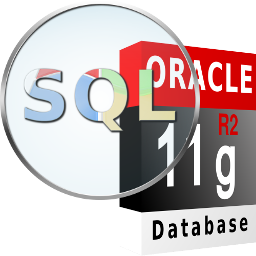
\includegraphics[scale=1]{ms_sql_oracle}}
  \ifthenelse{\boolparam} {
    \vspace{-1.5em}
  } {
    \vspace{-3.5em}
  }
  \begin{lrbox}{\litbox}
    \begin{minipage}{.96\linewidth}
}{
    \end{minipage}
  \end{lrbox}
  \usebox{\litbox}
  \par
  \ifthenelse{\boolparam} {
  \par
  \addvspace{\baselineskip}
  } {
  }
}

\newcommand{\kapitelnummer}[1]{
    \large\setlength{\vertspace}{-2.5em}
    \multiply\vertspace \value{#1}
    \rohead{
      \vspace{\vertspace}
      \large\colorbox{black}{\textcolor{white}{\thechapter\hspace{3mm}}}\hspace*{-5.8em}
    }
}

\newcommand{\identifier}[1]{\textsc{#1}}
\newcommand{\languageorasql}[1]{\lstinline[language=oracle_sql]{#1}}
\newcommand{\languagemssql}[1]{\lstinline[language=ms_sql]{#1}}
\newcommand{\languagerman}[1]{\lstinline[language=rman]{#1}}
\newcommand{\languageplsql}[1]{\lstinline[language=plsql]{#1}}
\newcommand{\languagesqlplus}[1]{\lstinline[language=sqlplus]{#1}}
\newcommand{\languageconfigfile}[1]{\lstinline[language=configfile]{#1}}
\newcommand{\languageexpdpimpdp}[1]{\lstinline[language=expdp_impdp]{#1}}
\newcommand{\languagepowershell}[1]{\lstinline[language=powershell]{#1}}
\newcommand{\oscommand}[1]{\texttt{#1}}
\newcommand{\privileg}[1]{\texttt{#1}}
\newcommand{\parameter}[1]{\MakeLowercase{\textsf{#1}}}

\newcommand{\pk}[1]{\underline{#1}}
\newcommand{\fk}[1]{$\Uparrow$#1$\Uparrow$}
\newcommand{\nn}[1]{#1 [NN]}
\newcommand{\un}[1]{#1 [UN]}

\newcommand{\SELECT}{\languageorasql{SELECT}}
\newcommand{\FROM}{\languageorasql{FROM}}
\newcommand{\WHERE}{\languageorasql{WHERE}}
\newcommand{\GROUPBY}{\languageorasql{GROUP BY}}
\newcommand{\HAVING}{\languageorasql{HAVING}}
\newcommand{\ORDERBY}{\languageorasql{ORDER BY}}
\newcommand{\CHECK}{\languageorasql{CHECK}}
\newcommand{\NOTNULL}{\languageorasql{NOT NULL}}
\newcommand{\UNIQUE}{\languageorasql{UNIQUE}}
\newcommand{\PRIMARYKEY}{\languageorasql{PRIMARY KEY}}
\newcommand{\FOREIGNKEY}{\languageorasql{FOREIGN KEY}}
\newcommand{\INSERT}{\languageorasql{INSERT}}
\newcommand{\UPDATE}{\languageorasql{UPDATE}}
\newcommand{\DELETE}{\languageorasql{DELETE}}
\newcommand{\COMMIT}{\languageorasql{COMMIT}}
\newcommand{\ROLLBACK}{\languageorasql{ROLLBACK}}
\newcommand{\GRANT}{\languageorasql{GRANT}}
\newcommand{\REVOKE}{\languageorasql{REVOKE}}
\newcommand{\DENY}{\languageorasql{DENY}}

\newcommand{\changefont}[3]{\fontfamily{#1} \fontseries{#2} \fontshape{#3} \selectfont}
\newcommand{\beispiel}[1]{\hyperref[#1]{Beispiel~\ref*{#1}}}
\newcommand{\abschnitt}[1]{\hyperref[#1]{Abschnitt~\ref*{#1}}}
\newcommand{\tabelle}[1]{\hyperref[#1]{Tabelle~\ref*{#1}}}
\newcommand{\abbildung}[1]{\hyperref[#1]{Abbildung~\ref*{#1}}}
\makeatletter
\newcommand{\myhref}[2]{\hyper@linkurl{#2}{#1}}
\makeatother
